\documentclass[a4paper, 12pt, titlepage, oneside]{article}
\usepackage[utf8]{inputenc}
\usepackage[czech]{babel}
\usepackage[total={18.5cm,25cm}, top=3cm, left=1.25cm, includefoot]{geometry}
\usepackage[T1]{fontenc}
\usepackage{amsmath}
\usepackage{amsfonts}
\usepackage{amssymb}

\usepackage{fancyhdr}
\usepackage{amsmath} % větší zlomyk pmocí \dfrac
\usepackage{graphicx} % vkládání obrázků
\usepackage{float} % H aby bloky neuplavali
\usepackage{ctable} % horozontální čára s nastavitelnou šířkou a mezerami od okolí

\usepackage{pdfpages} % vložení pdf stránky

% záhlaví a zápatí ----------------------------------------------------------------
\pagestyle{fancy}
\fancyhf{}
% jednostranná sazba
\fancyhead[R]{Jan \textsc{Vykydal} 4A}
\fancyhead[L]{SDR Software Defined Radio}
\fancyfoot[C]{\thepage/\pageref{konec}}
\renewcommand{\headrulewidth}{0.4pt}
\renewcommand{\footrulewidth}{0.4pt}

%\renewcommand{\figurename}{Obrázek č.}
%\renewcommand{\tablename}{Tabulka č.}

%\renewcommand{\contentsname}{Obsah} 
%\renewcommand{\listfigurename}{Seznam obrázků} 
%\renewcommand{\listtablename}{Seznam tabulek} 




\newcommand{\HRule}{\rule{\linewidth}{0.5mm}}

\setcounter{page}{1}


\begin{document}

	\begin{titlepage}
  \begin{center}

  % Upper part of the page. The '~' is needed because \\
  % only works if a paragraph has started.
  %
\includegraphics[width=0.15\textwidth]{./logo}~\\[1cm]

  \textsc{\LARGE Vyšší odborná škola a Střední průmyslová škola elektrotechnická Olomouc}%\\[1.5cm]

	% logo školy
	\begin{figure}[H]
    \centering
    
\includegraphics[width=4cm]{img/logo/logo.pdf}
  \end{figure}

  \textsc{\Large STŘEDOŠKOLSKÁ ODBORNÁ ČINNOST}\\[0.5cm]
  Obor 10. elektrotechnika, elektronika a telekomunikace\\[.2cm]
	
	
	
  % Title
  \HRule \\[0.4cm]
  { \huge \bfseries SDR přijímač pro pásmo KV\\[0.4cm] }

  \HRule \\[.5cm]
  
  SDR RECEIVER FOR SW BAND\\[1.5cm]
		
  % Author and supervisor
  \emph{Autor:} Jan \textsc{Vykydal}
  
  \vfill

  % Bottom of the page
  {\large \today}

  \end{center}
\end{titlepage}

	\clearpage
	\tableofcontents
	\listoftables
	\listoffigures
	\clearpage
	\section*{Úvod}
\addcontentsline{toc}{section}{Úvod} 
\indent\indent Cílem mé práce bylo navrhnout a realizovat SDR přijímač pro pásmo krátkých vln. Toto téma spojuje mikroprocesorovou a číslicovou techniku s radioelektronikou, kterou jsem si chtěl osahat. V úvodu bych chtěl dále vysvětlit, co se skrývá za zkratkou SDR.

Zkratka SDR znamená Software Defined Radio (v překladu Softwarově Definované Rádio). Jedná se o další vývojovou etapu rádiových přijímačů a vysílačů. Klasická analogová rádia se postupně vyvíjela od jednoduchých krystalových přijímačů s přímým zesílením, přes přímosměšující tranzistorové přijímače až k velmi složitým přijímačům typu superheterodyn s možnostmi přepínání nejrůznějších demodulací a velkým rozsahem přijímaných pásem. Tyto přijímače ale začínaly být tak složité, že se k napěťovým signálům nesoucím informace při jejich zpracování přičítal šum jednotlivých bloků. Tento šum pak výrazně zhoršoval kvalitu přijímaného signálu. SDR je moderní technologie, která se snaží tyto nežádoucí vlivy hardwarových komponentů omezit. Ideální SDR přijímač se skládá jen z antény analogově digitálního převodníku a digitálního obvodu, který signál demoduluje. Díky tomu se k přijímané informaci přidává jen minimální chyba při digitalizaci signálu. Tato technologie tedy posouvá zařízení pro rádiový přenos o světelné roky dál, jelikož je s jejich pomocí možné přenášet v podstatě libovolně modulovaný signál, a tím pak přenášet komprimované informace, nebo vytvářet nové digitální modulace. Obrovskou výhodou SDR přijímačů a vysílačů je jejich neustálé vylepšování bez nutnosti jakkoliv měnit hardware přijímače.
\begin{figure}[H]
	\centering
	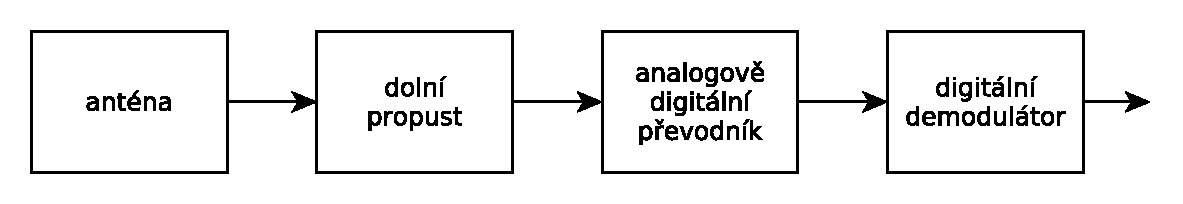
\includegraphics[width=170mm]{img/i_sdr.pdf}
	\caption{blokové schéma ideálního SDR přijímače}    		
\end{figure}

\clearpage
		
	
  		
  		
	\section{Schéma zapojení LNA}
	LNA Low Noise Amplifer, neboli nízkošumový zesilovač, je zesilovač určený k zesílení signálu z antény. tento zesilovač je selektivní, díky vstupnímu filtru pásmové propusti. Tento elektronický obvod tedy do značné míry určuje možnosti zařízení.
	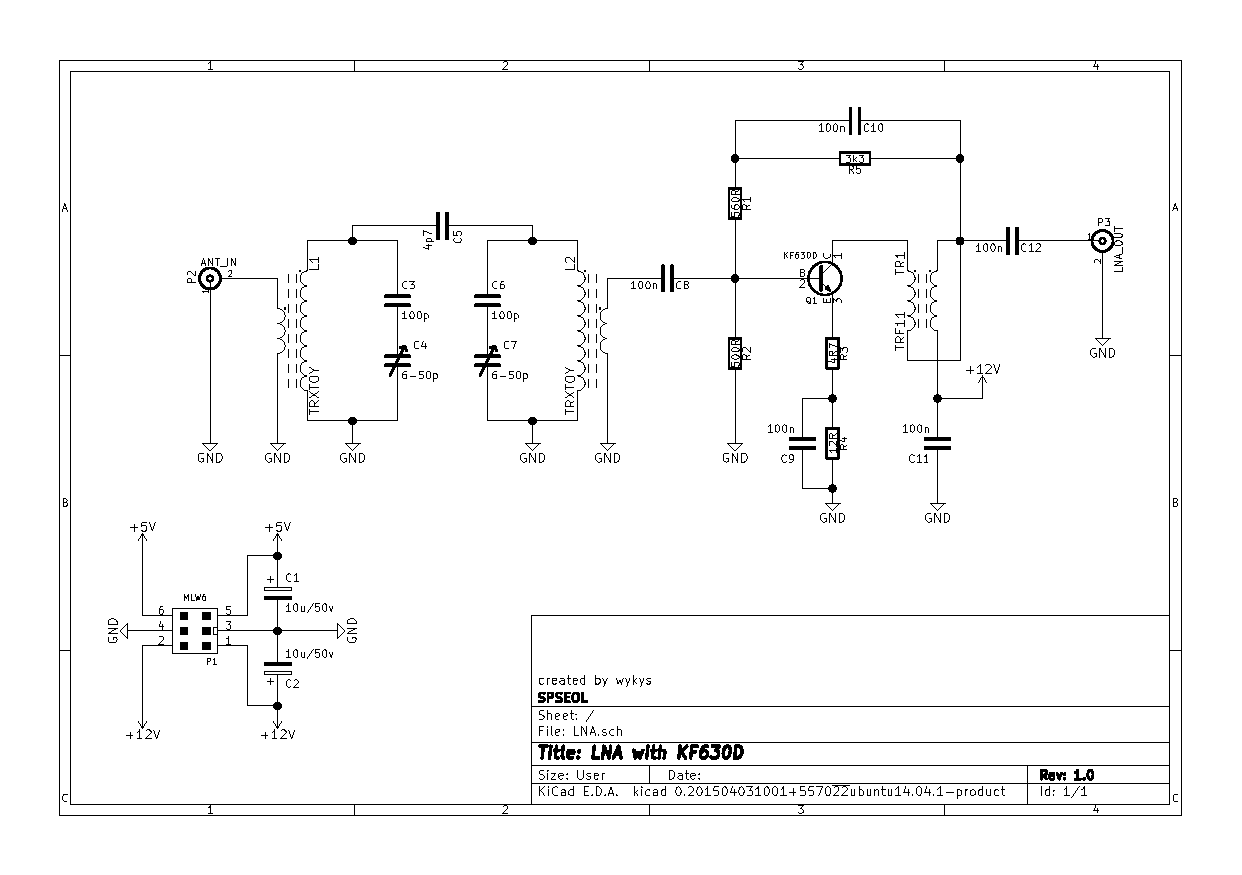
\includepdf[landscape=true]{img/LNA.pdf}
	
\section{Schéma zapojení DDS}
	Schéma je rozděleno do tří bloků v levé horní části se nachází stabilizátor 3V3 pro křemíkový oscilátor a Kondenzátory pro vyrovnání nárazových odběrů. V levé dolní části je digitální část DDS, popisováno z leva do prava: konektor pro konfigurování DDSky, oddělovací buffer 74F245, jehož výstupy jdou do DDSky. Nahoře je již zmíněný křemíkový oscilátor a tvarovač impulsů. V pravé horní části se nachází VF část tvořená dolní propustí určené k potlačení vyšších harmonických z DAC. a Výkonový zesilovač tvořený tranzistorem KF630D s I$_c$ nastaveným na $20~mA$. Ke kolektoru tranzistoru je připojeno trafo, které je vinuto bifilárně a slouží k transformaci impedance na cca $50~\Omega$.
	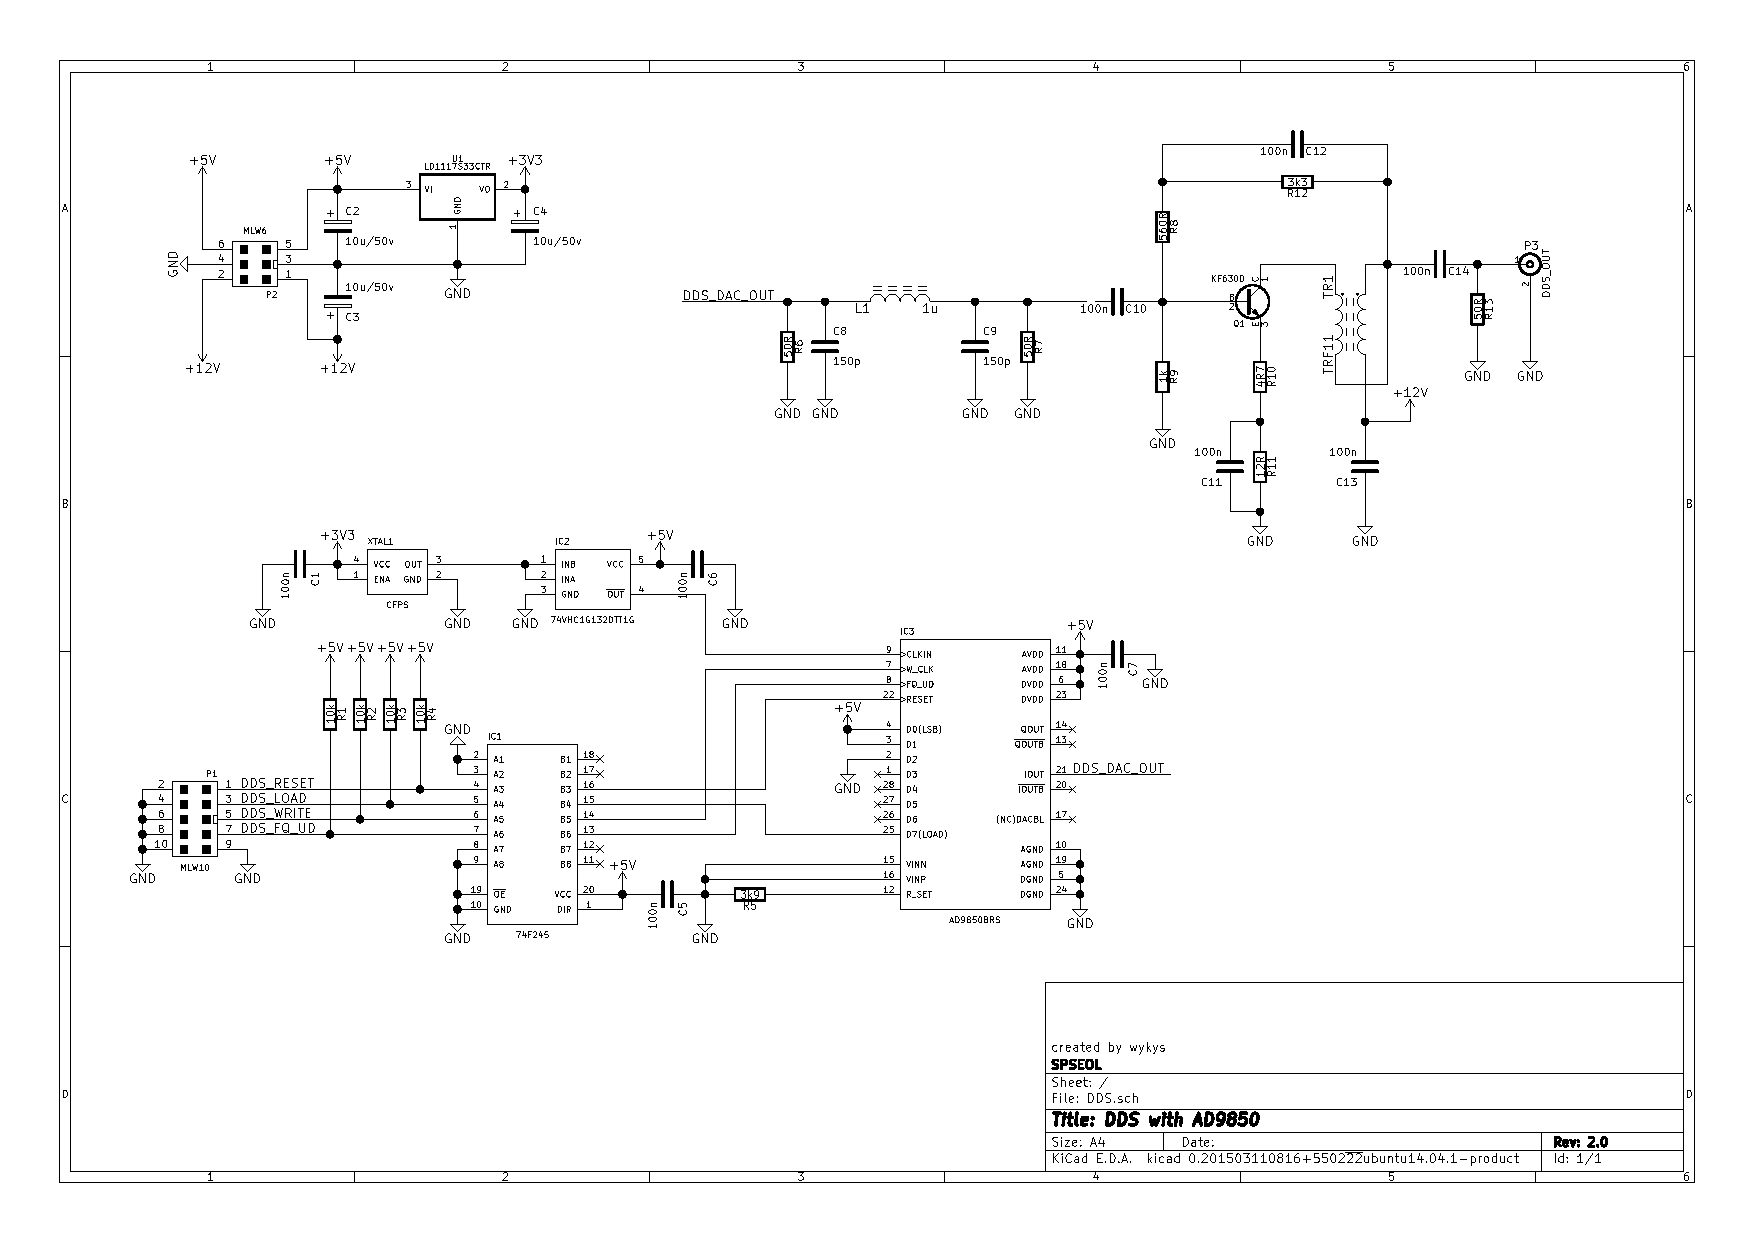
\includepdf[landscape=true]{img/DDS.pdf}
	
\section{Schéma zapojení řídící deska}
	Řídící deska slouží k řízení výstupní frekvence lokálního oscilátoru založeného na DDS. A nastavování pořadované výstuúní frekvence slouží enkoder. Dále je na desce připraven konektor pro USART, aby bylo možné řídit i řídíví desku s nadřazeného počítače. Dále desky zobraduje příjmanou stanici na znakový LCD disply. Zobrazovaná frekvence je absolutní hodnota zordílu frekvence lokálního oscilátoru a mezifrekvence.
	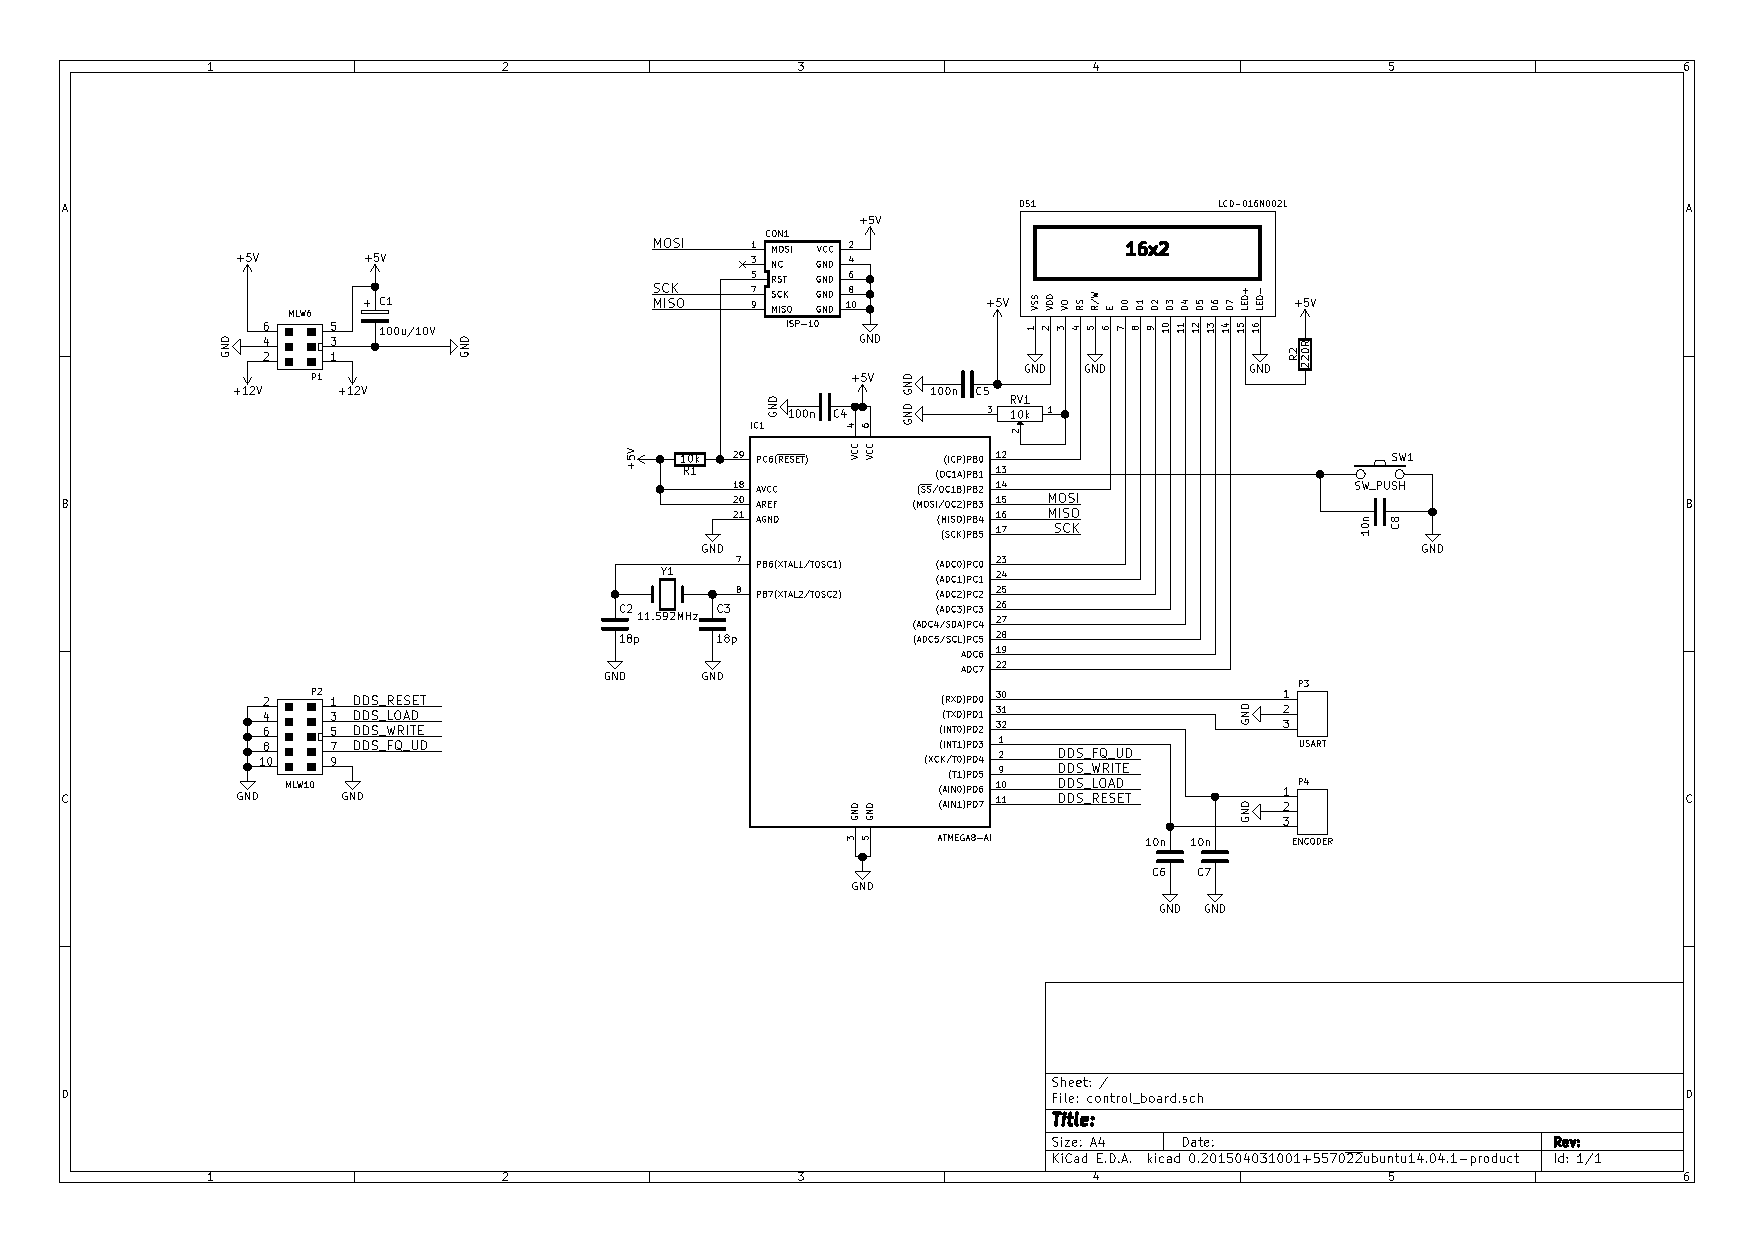
\includepdf[landscape=true]{img/control_board.pdf}
	
\section{Schéma zapojení mixer}
	Tento obvod slouží k převedení signálu do základního pásma. K tomu používá dvou směšovaců. Klasického kruhového diodového směčovaře pro převod na mezifrekvenci $6~MHz$ a tzv. Tayloe kvadraturní detektor, který generuje signály I a Q navzájem posunuté o $\frac{\pi}{2}$.
	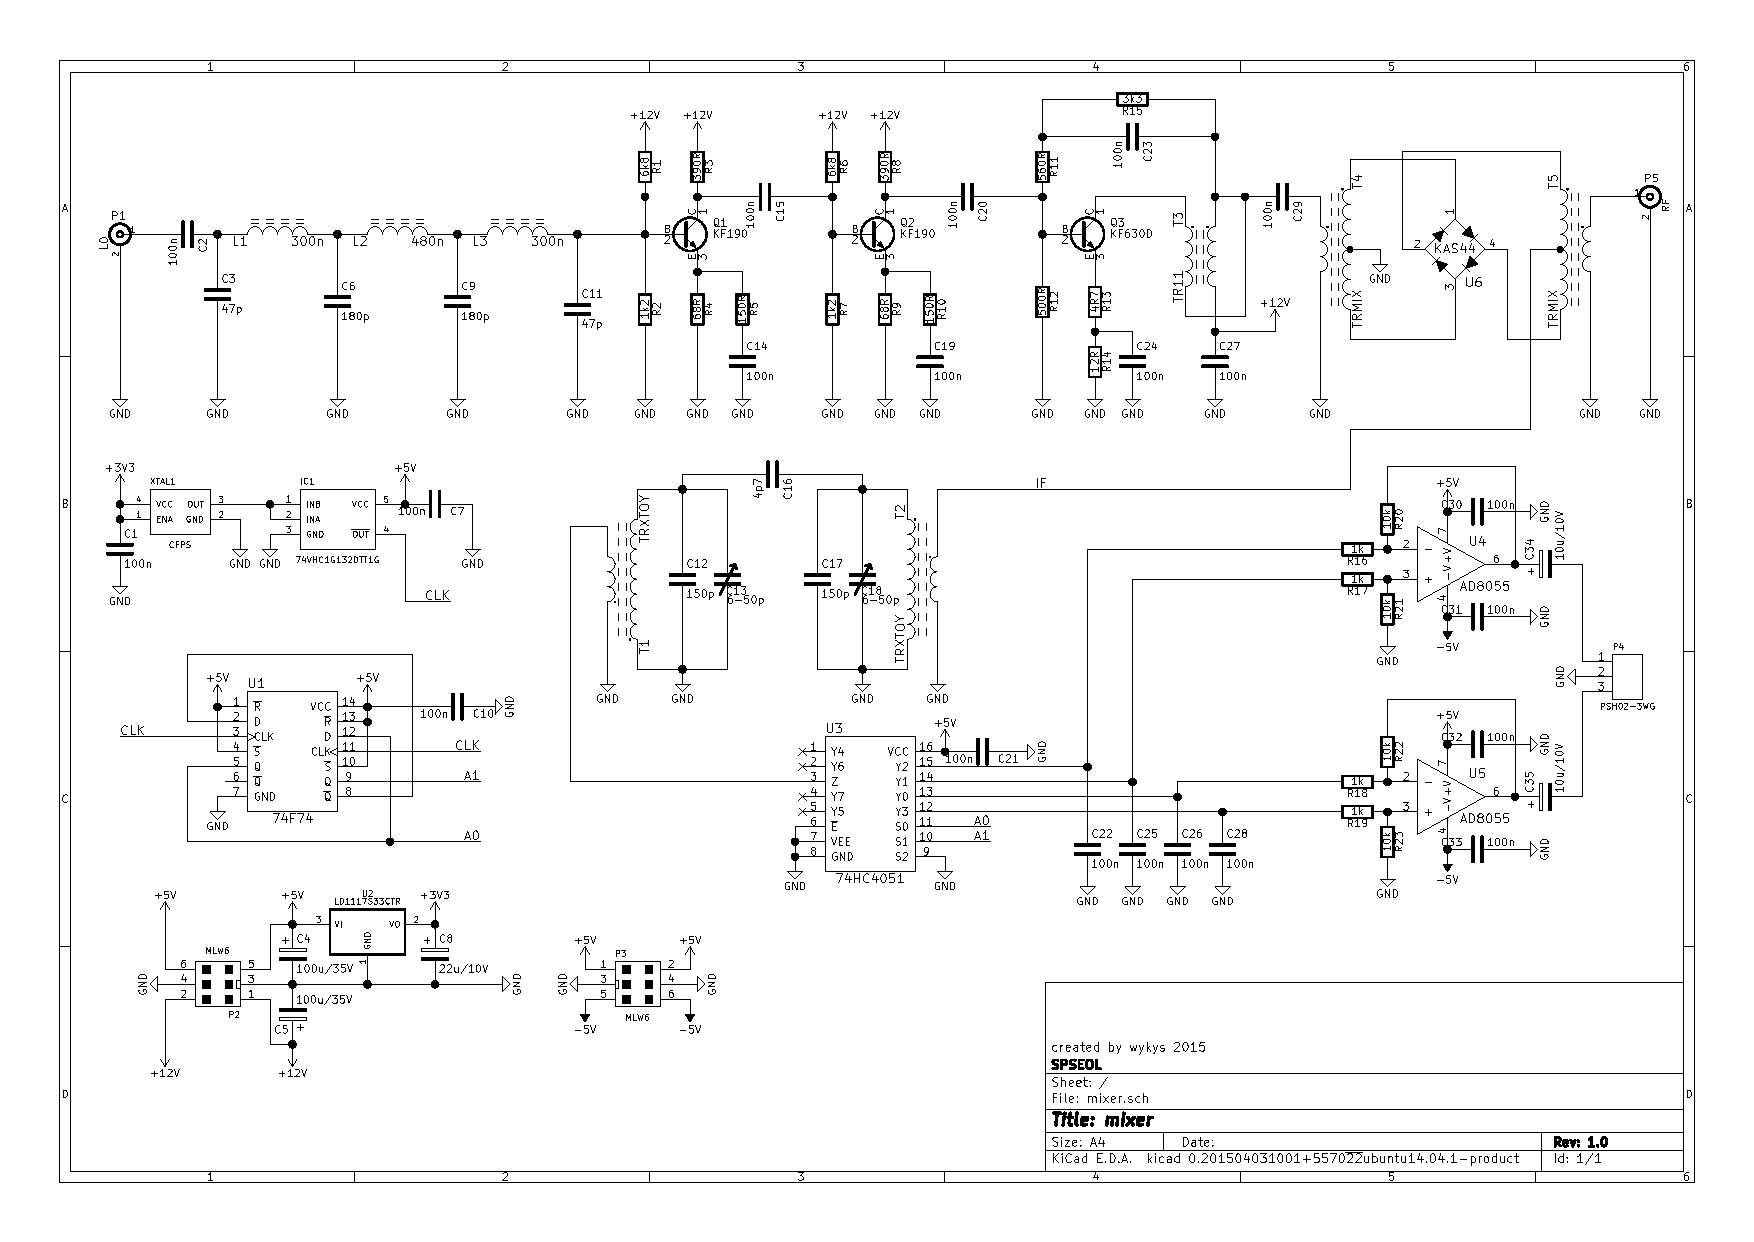
\includepdf[landscape=true]{img/mixer.pdf}
	
\section{Schéma zapojení zdroj}
	Zdroj slouží k napájení celého zařízení poskytuje symetrické napětí $5~V$ a napěří $12~V$.
	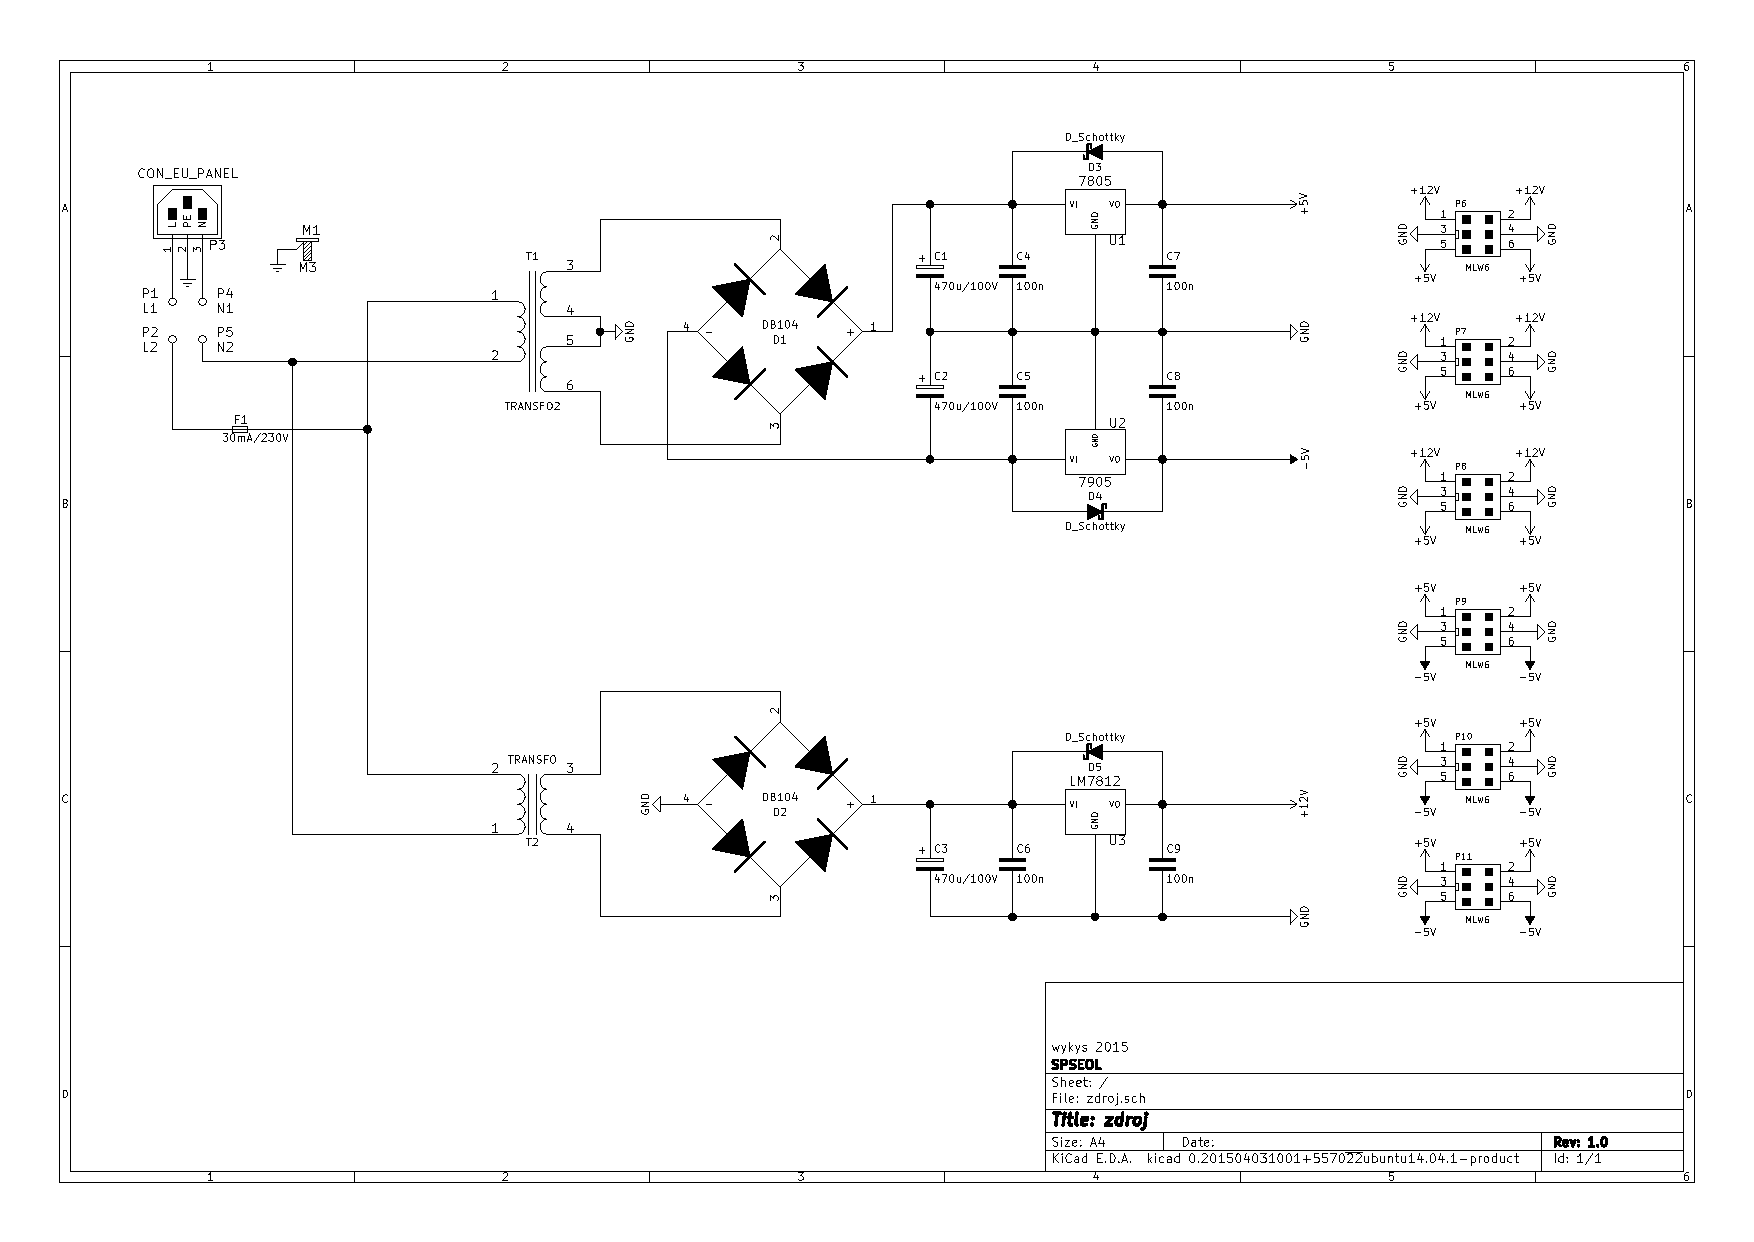
\includepdf[landscape=true]{img/zdroj.pdf}
	\section{Plošný spoj}
	% blokáč AD9850
	\begin{figure}[H]
    	\centering
    	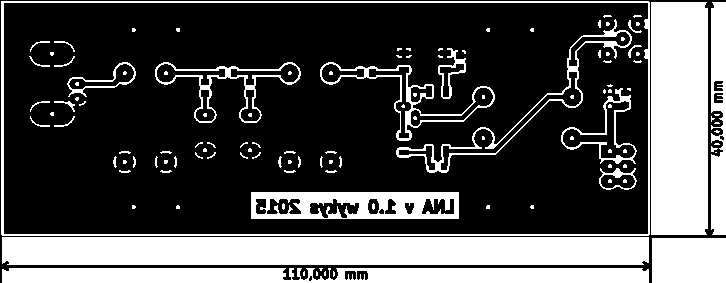
\includegraphics[width=160mm]{img/LNA-brd.pdf}
    	\caption{DPS LNA}    		
  	\end{figure}
  	
  	\begin{figure}[H]
    	\centering
    	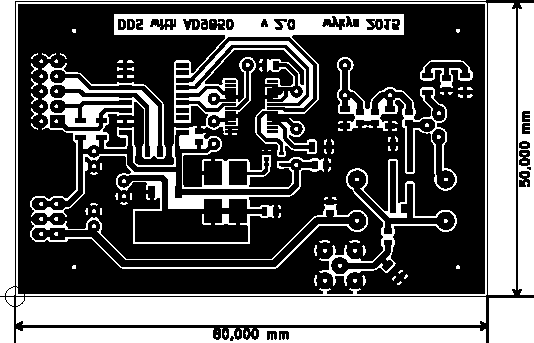
\includegraphics[width=160mm]{img/DDS-brd.pdf}
    	\caption{DPS DDS}    		
  	\end{figure}
  	
  	\begin{figure}[H]
    	\centering
    	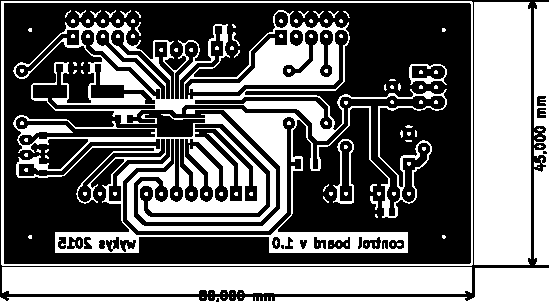
\includegraphics[width=160mm]{img/control_board-brd.pdf}
    	\caption{DPS řídící deska}    		
  	\end{figure}
  	
  	\begin{figure}[H]
    	\centering
    	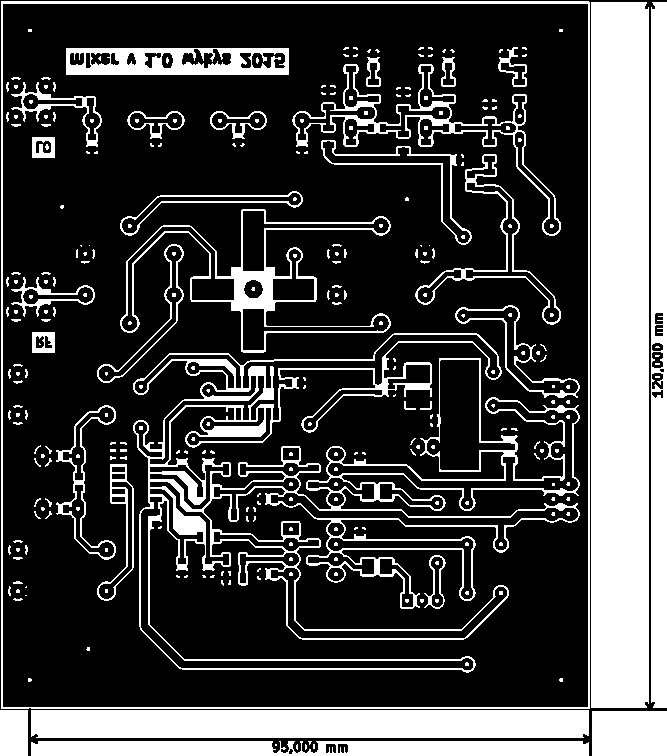
\includegraphics[width=160mm]{img/mixer-brd.pdf}
    	\caption{DPS mixer}    		
  	\end{figure}
  	
  	\begin{figure}[H]
    	\centering
    	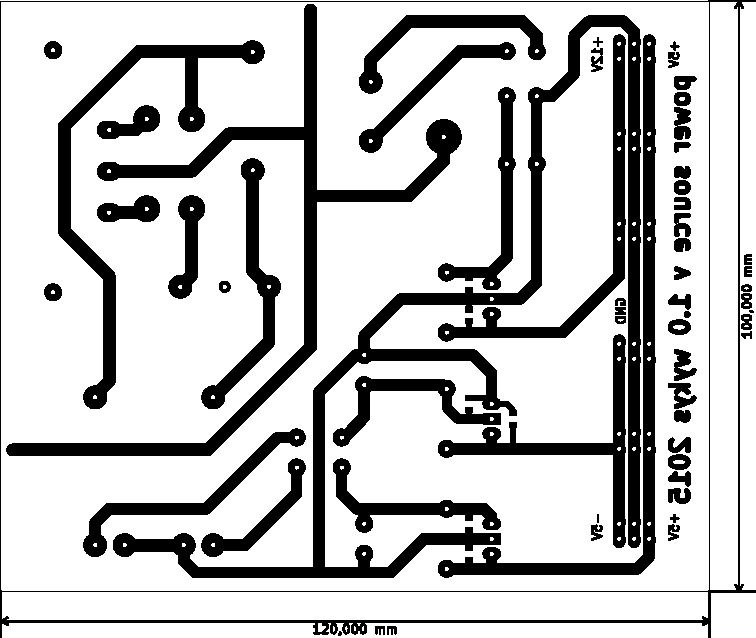
\includegraphics[width=160mm]{img/zdroj-brd.pdf}
    	\caption{DPS zdroj}    		
  	\end{figure}
  	
  	% blokáč AD9850
	\begin{figure}[H]
    	\centering
    	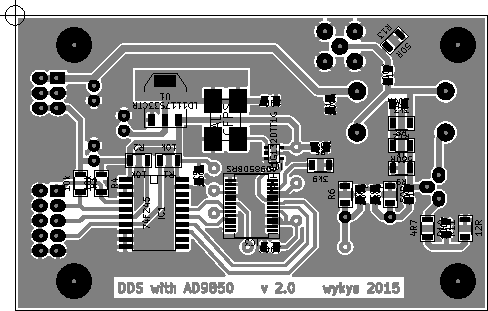
\includegraphics[width=180mm]{img/ob.pdf}
    	\caption{Osazovák vrstva mědi}    		
  	\end{figure}
  	
  	% blokáč AD9850
	\begin{figure}[H]
    	\centering
    	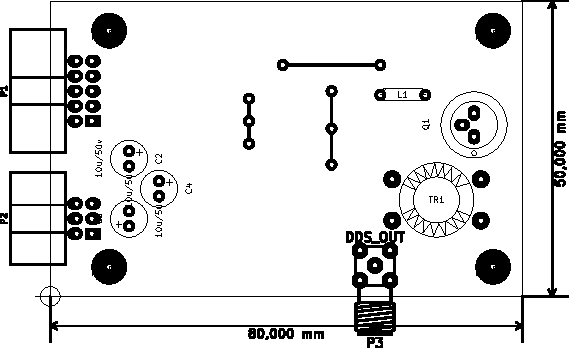
\includegraphics[width=180mm]{img/ot.pdf}
    	\caption{Osazovák horní vrstva}    		
  	\end{figure}
	\section{Seznam součástek}
	

	\begin{table}[H]
		\begin{center}
			\begin{tabular}[H]{!{\vrule width 1pt}c|c|c|c!{\vrule width 1pt}}
			    \specialrule{1pt}{0pt}{0pt} 
			    \textbf{Určovatel}	&	\textbf{Pouzdro}	&	\textbf{Množství}	&	\textbf{Určení}	\\\specialrule{1pt}{0pt}{0pt} 
				C1,C5,C6,C7,C10,C11,C12,C13,C14	&	SMD-0805	&	9	&	100n	\\\hline
				C2,C3,C4	&	11.2x6.3mm\_RM2.5	&	3	&	10u/50v	\\\hline
				C8,C9	&	SMD-0805	&	2	&	150p	\\\hline
				IC1	&	SO-20-L	&	1	&	74F245	\\\hline
				IC2	&	SOT-23-5	&	1	&	74VHC1G132DTT1G	\\\hline
				L1	&	R3-LARGE\_PADS	&	1	&	1u	\\\hline
				Q1	&	OldSowjetaera	&	1	&	KF630D	\\\hline
				R1,R2,R3,R4	&	R\_1206	&	4	&	10k	\\\hline
				R5	&	R\_1206	&	1	&	3k9	\\\hline
				R6,R7,R13	&	R\_1206	&	3	&	50R (2*100R)	\\\hline
				R8	&	R\_1206	&	1	&	560R	\\\hline
				R9	&	R\_1206	&	1	&	1k	\\\hline
				R10	&	R\_1206	&	1	&	4R7	\\\hline
				R11	&	R\_1206	&	1	&	12R	\\\hline
				R12	&	R\_1206	&	1	&	3k3	\\\hline
				TR1	&	Amidon-T44	&	1	&	TRF11	\\\hline
				U1	&	SOT-223	&	1	&	LD1117S33CTR	\\\hline
				P3	&	sma\_90\_r300.124.403	&	1	&	DDS\_OUT	\\\hline
				P1	&	vasch\_strip\_5x2\_90	&	1	&	MLW10	\\\hline
				P2	&	vasch\_strip\_3x2\_90	&	1	&	MLW6	\\\hline
				$-$	&	M3	&	4	&	M3	\\\hline
				IC3	&	SSOP-28 &	1	&	AD9850BRS	\\\hline
				XTAL1	&	SMD7x5	&	1	&	CFPS
				\\\specialrule{1pt}{0pt}{0pt} 

			\end{tabular}

			\caption{Tabulka použitých součástek pro desku DDS, ostatní zde nebyli uvedeny z důvodu nedostatku papíru}
			\label{tab:s1}      
		\end{center}
	\end{table}
	\section{Použití zařízení}
	Zařízení je určeno pro příjem KV vysílení na pásmu dvacet metrů, lokální oscilátor jde ale přeladit a tak se dá sice se znatelným útlumem použít i pro příjem v jiných pásmech. Dále se dá zařízení použít na vývoj algoritmů zpracování signálu.
	\label{konec}

\end{document}